%%%%%%%%%%%%%%%%%%%%%%%%%%%%%
%Since : 2018/11/13
%Update: <2019/02/18>
% -*- coding: utf-8 -*-
%%%%%%%%%%%%%%%%%%%%%%%%%%%%%
\documentclass[12pt, a4j]{jreport}
\usepackage[dvipdfmx]{graphicx}
%\usepackage{graphicx}
\usepackage{amsmath}
\usepackage{amssymb}
\usepackage{cite}

\renewcommand{\prechaptername}{第}
\renewcommand{\postchaptername}{回}
\renewcommand{\thesection}{\arabic{section}}

\title{Excelによる統計処理実習}
\author{公立小松大学臨床工学科 \\ 藤田 一寿}
\date{}

\begin{document}

\maketitle

\chapter{Excelによる統計処理実習1}

\section{目的}

Excelの操作を通し,データ処理の基礎とグラフの作成の仕方を学ぶ.

\section{理論}

\subsection{統計とは}


全体の特徴を捉える.

サンプル

統計量

総和


平均
\begin{equation}
    \mu = \frac{1}{N} \sum_{i=1}{N}
\end{equation}


分散
\begin{equation}
    \sigma^2 = \frac{1}{N} \sum_{i=1}{N} (x - \mu)^2
\end{equation}

ヒストグラム

\section{Excel実験}

\subsection{総和,平均,分散}

エクセルでの総和の計算.

\begin{enumerate}
    \item 総和を表示したいセルを選択する.
    \item ``=sum(''と入力する.
    \item 総和を計算したいセルを選択する.そうすると``(''の後ろにセル番号が入力される(図\ref{fig:sum}).
    \item )を入力する.
\end{enumerate}

\begin{figure}[htbp]
  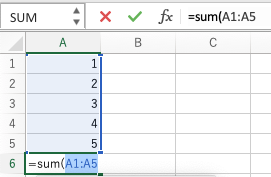
\includegraphics[width=10cm]{sum.png}
  \caption{総和を計算したいセルを選択した状態.}
  \label{fig:sum}
\end{figure}


\paragraph{演習}
csvの平均,分散を求めよ.

csvをヒストグラムにせよ.
標本分散の期待値を求めよ.
折れ線グラフ.
散布図をかけ.
相関係数を求めよ.

\section{考察}


\section{おまけ}

確率分布

ガウス分布

R,python

プロット
R,matplotlib,gnuplot


有料ならmatlabがある.

\chapter{Excelによる統計処理実習2}

\section{目的}

\section{原理}

散布図

回帰直線

相関係数

不偏分散

\section{実験}

不偏分散

\section{考察}


\section{レポートの出し方}

提出はpdf,docxなどの電子データで送る.



\end{document}
